The motor equation (\ref{eq:fin}) gives an expression for the motor torques, however the system dynamics are defined in terms of geometric joint angles. The inclusion of differential drive systems means that the joint angles, $\gamma$, do not directly correspond to motor rotations, $\theta$, as shown in \emph{Figure \ref{fig:motorloc}}.


\begin{figure}[htp]
  \center
  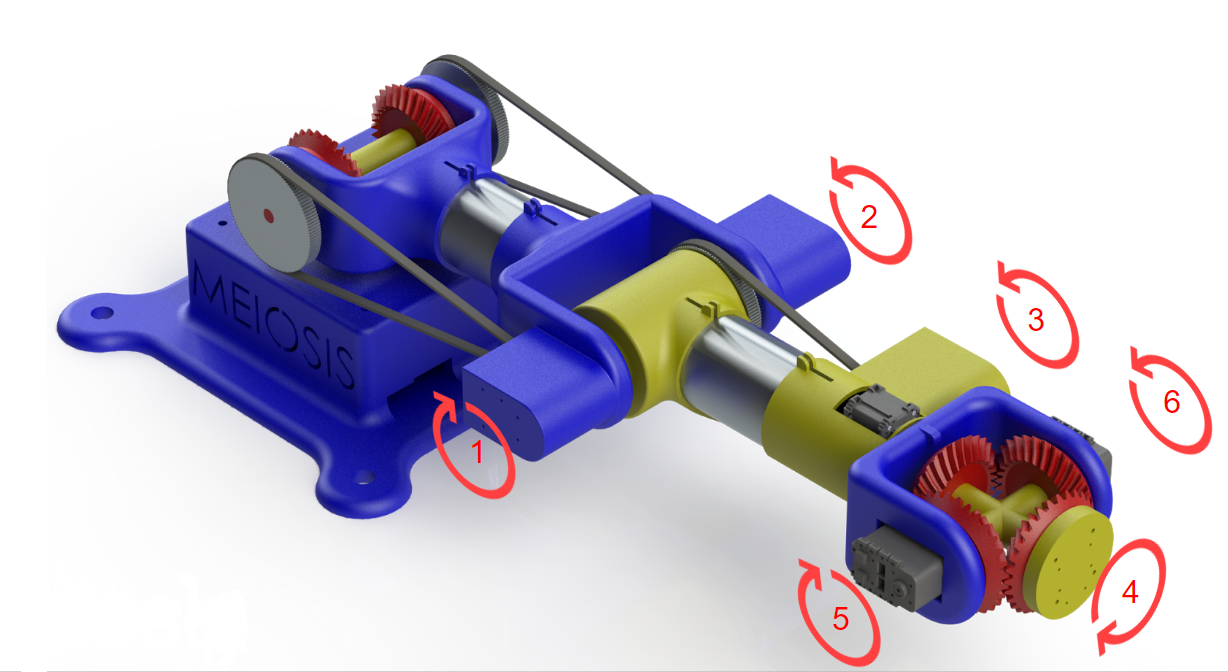
\includegraphics[width=.75\textwidth,frame]{motorloc}
  \caption{Motor Locations and Orientations}
  \label{fig:motorloc}
\end{figure}

\emph{Figure \ref{fig:motorloc}} shows the motor positions and relative orientations.
This layout was used to define a linear relation between the joint angles and the motor rotations, described in equation (\ref{eq:A}).

\begin{equation}
  \gamma = A\theta\quad \text{where}~~A=\left[\begin{array}{cccccc}
  -1/20 & 0 & {0} & {0} & {0} & {0} \\
   0 & -1/39 & {0} & {0} & {0} & {0} \\
    {0} & {0} & -1/39 & {0} & {0} & {0} \\
    {0} & {0} & {0} & -1/20 & {0} & {0} \\
     {0} & {0} & {0} & {0} & -1/20 & 0\\
      {0} & {0} & {0} & {0} & 0 & -1/20
    \end{array}\right]
\label{eq:A}
\end{equation}
Equation (\ref{eq:A}) can be used to map the joint angles to the motor angles. The gear ratio of 1:10 is represented by the variable N. Similarly, the motor angles can be determined by multiplying both sides of equation (\ref{eq:A}) by the inverse of matrix A, giving the following relation.
\begin{equation}
\theta=A^{-1} \gamma
\label{eq:Ainv}
\end{equation}
It is important to note that the virtual work done by the joint torques ($F_{\gamma}$) and the virtual work done by the motor torques ($F_{\theta}$) are equal. Using equation (\ref{eq:Ainv}), a linear relation between the joint torques and motor torques can be determined.
\[
\begin{aligned}
  \delta W = F_{\theta}^{T} \delta \theta&=F_{\gamma}^{T} \delta \gamma, \text { where } \delta \gamma=A \delta \theta \\
  F_{\theta}^{T} \delta \theta &= F_{\gamma}^{T}(A \delta \theta) \\
  F_{\theta}^{T}&=F_{\gamma}^{T} A\\
  \left(F_{\theta}^{T}\right)^{T}&=\left(F_{\gamma}^{T} A\right)^{T}\\
  F_{\theta}=A^{T} F_{\gamma} &\Leftrightarrow F_{\gamma}=A^{-T} F_{\theta}\qquad\quad
\end{aligned}
\]
Using this equation, a relation can be determined between the motor dynamics and the system dynamics given in equation (\ref{eq:fin}) and equation (\ref{eq:eoms}) respectively.

\[
H(\gamma) \ddot{\gamma}+d(\gamma, \dot{\gamma})+G(\gamma)=-A^{-T}\left(C_1A^{-1} \ddot{\gamma}+C_2 A^{-1} \dot{\gamma}+C_3 \theta_{d}- C_3A^{-1} \gamma\right)
\]
\begin{equation}
\ddot{\gamma}=H(\gamma)^{-1}\left(-A^{-T}\left(C_1 A^{-1} \ddot{\gamma}+C_2 A^{-1} \dot{\gamma}+C_3 \theta_{d}-C_3A^{-1} \gamma\right)-d(\gamma, \dot{\gamma})-G(\gamma)\right)
\label{eq:gddot}
\end{equation}

Because this equation includes the motor model, which in turn includes an internal PD controller, this equation can be integrated to solve for the system response given a desired motor angle input, $\theta_d$. However, doing so will not result in the desired system response. This control scheme does not have any compensation for the inertia of the links, and it is also lacking gravity compensation. This can be remedied by modifying the input to the motors, $\theta_d$. A new input, $u$, is defined such that gravity can be compensated. Thus, the motor input term in equation (\ref{eq:gddot}) must include both compensation for gravity and the desired motor angle.
\[
A^{-T} C_3  u=G(\gamma)+d(\gamma, \dot{\gamma})+A^{-T} C_3\theta_{d}
\]
\begin{equation}
u=\left(A^{-T} C_3\right)^{-1} \left(G(\gamma)+d(\gamma, \dot{\gamma})\right) + \theta_{d}
\end{equation}
With this new motor input, the closed loop control system equations of motion are given as:
\begin{equation}
\ddot{\gamma}=H(\gamma)^{-1}\left(-A^{-T}\left(C_1 A^{-1} \ddot{\gamma}+C_2 A^{-1} \dot{\gamma}+C_3 u-C_3A^{-1} \gamma\right)-d(\gamma, \dot{\gamma})-G(\gamma)\right)
\label{eq:gddotfin}
\end{equation}
Equation (\ref{eq:gddotfin}) can then be integrated to solve for the system response given desired motor angles.

% \begin{figure}[htp]
%   \center
%   \begin{subfigure}[c]{0.33\textwidth}
%     \center
%     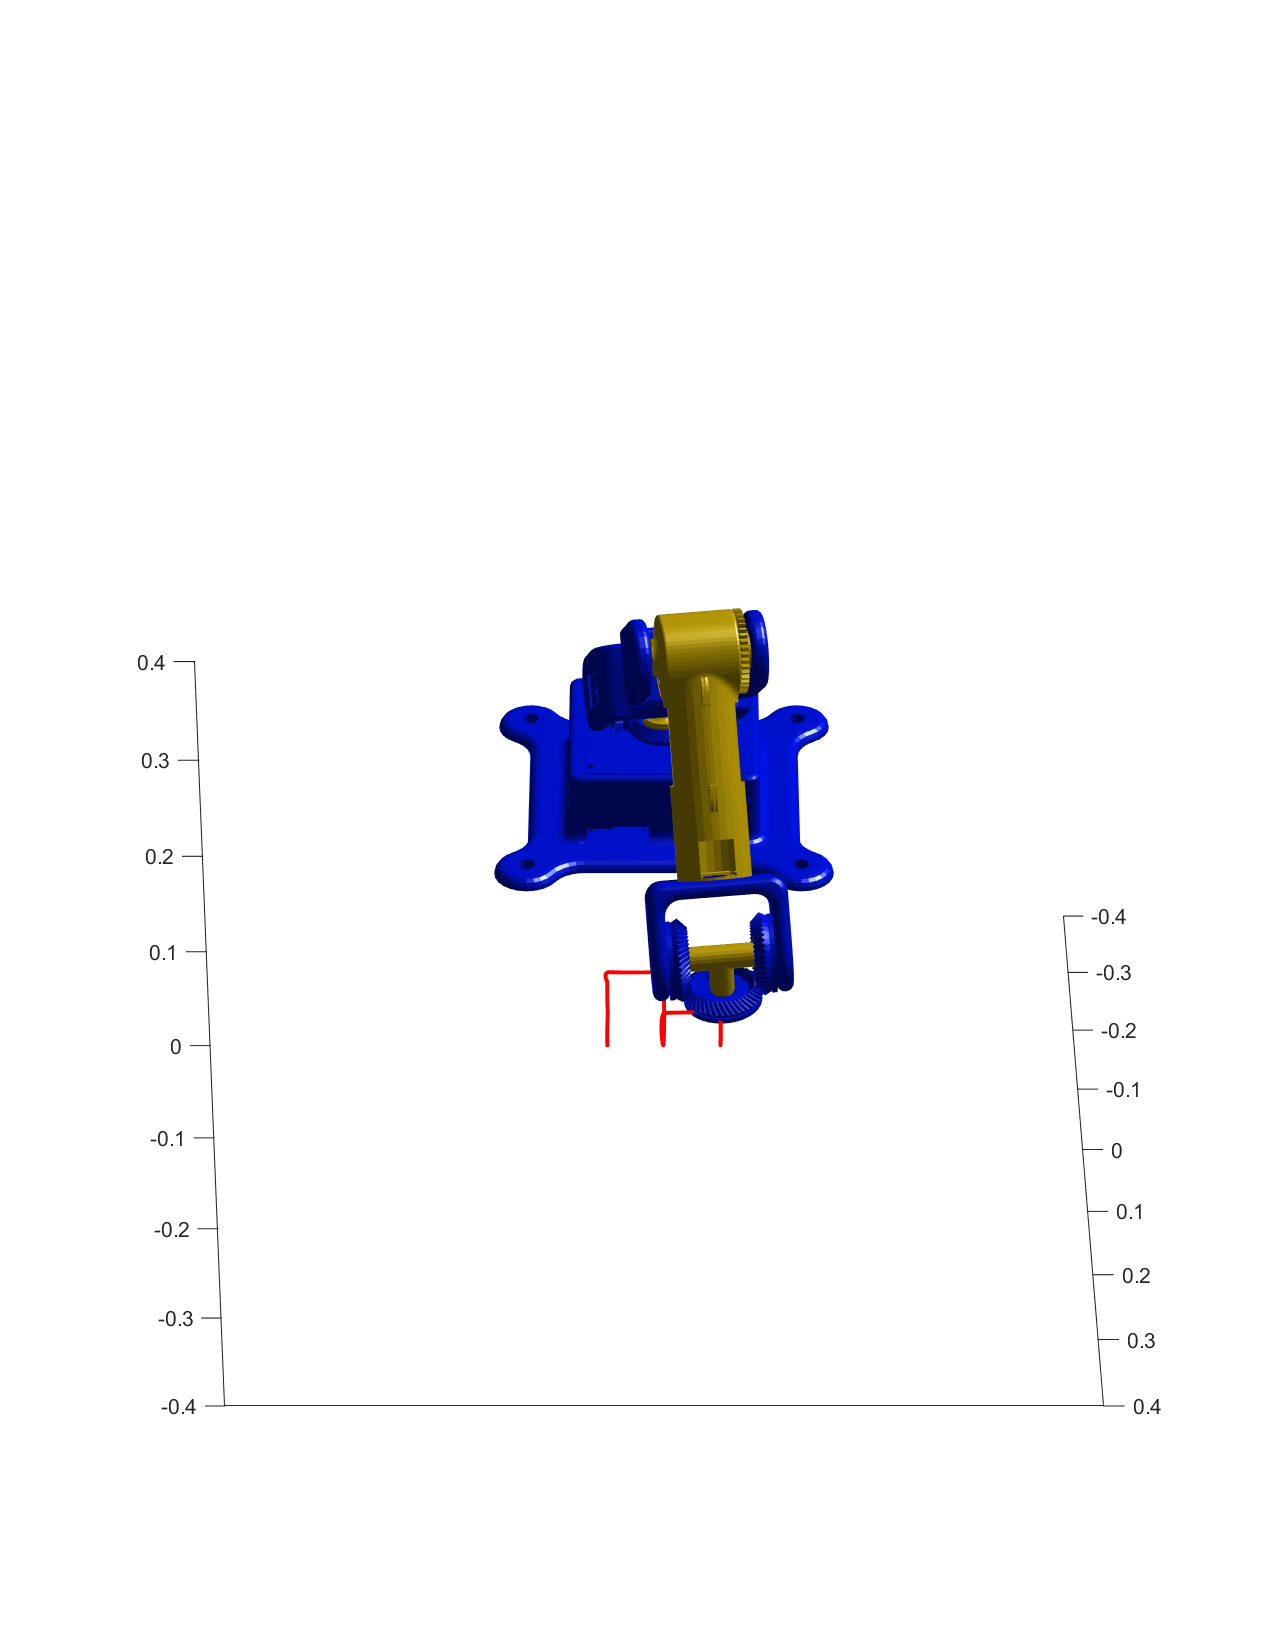
\includegraphics[width=.9\textwidth,frame]{clsnap1}
%     \caption{Frame Snapshot near Simulation \\Initiation}
%   \end{subfigure}%
%   \begin{subfigure}[c]{0.33\textwidth}
%     \center
%     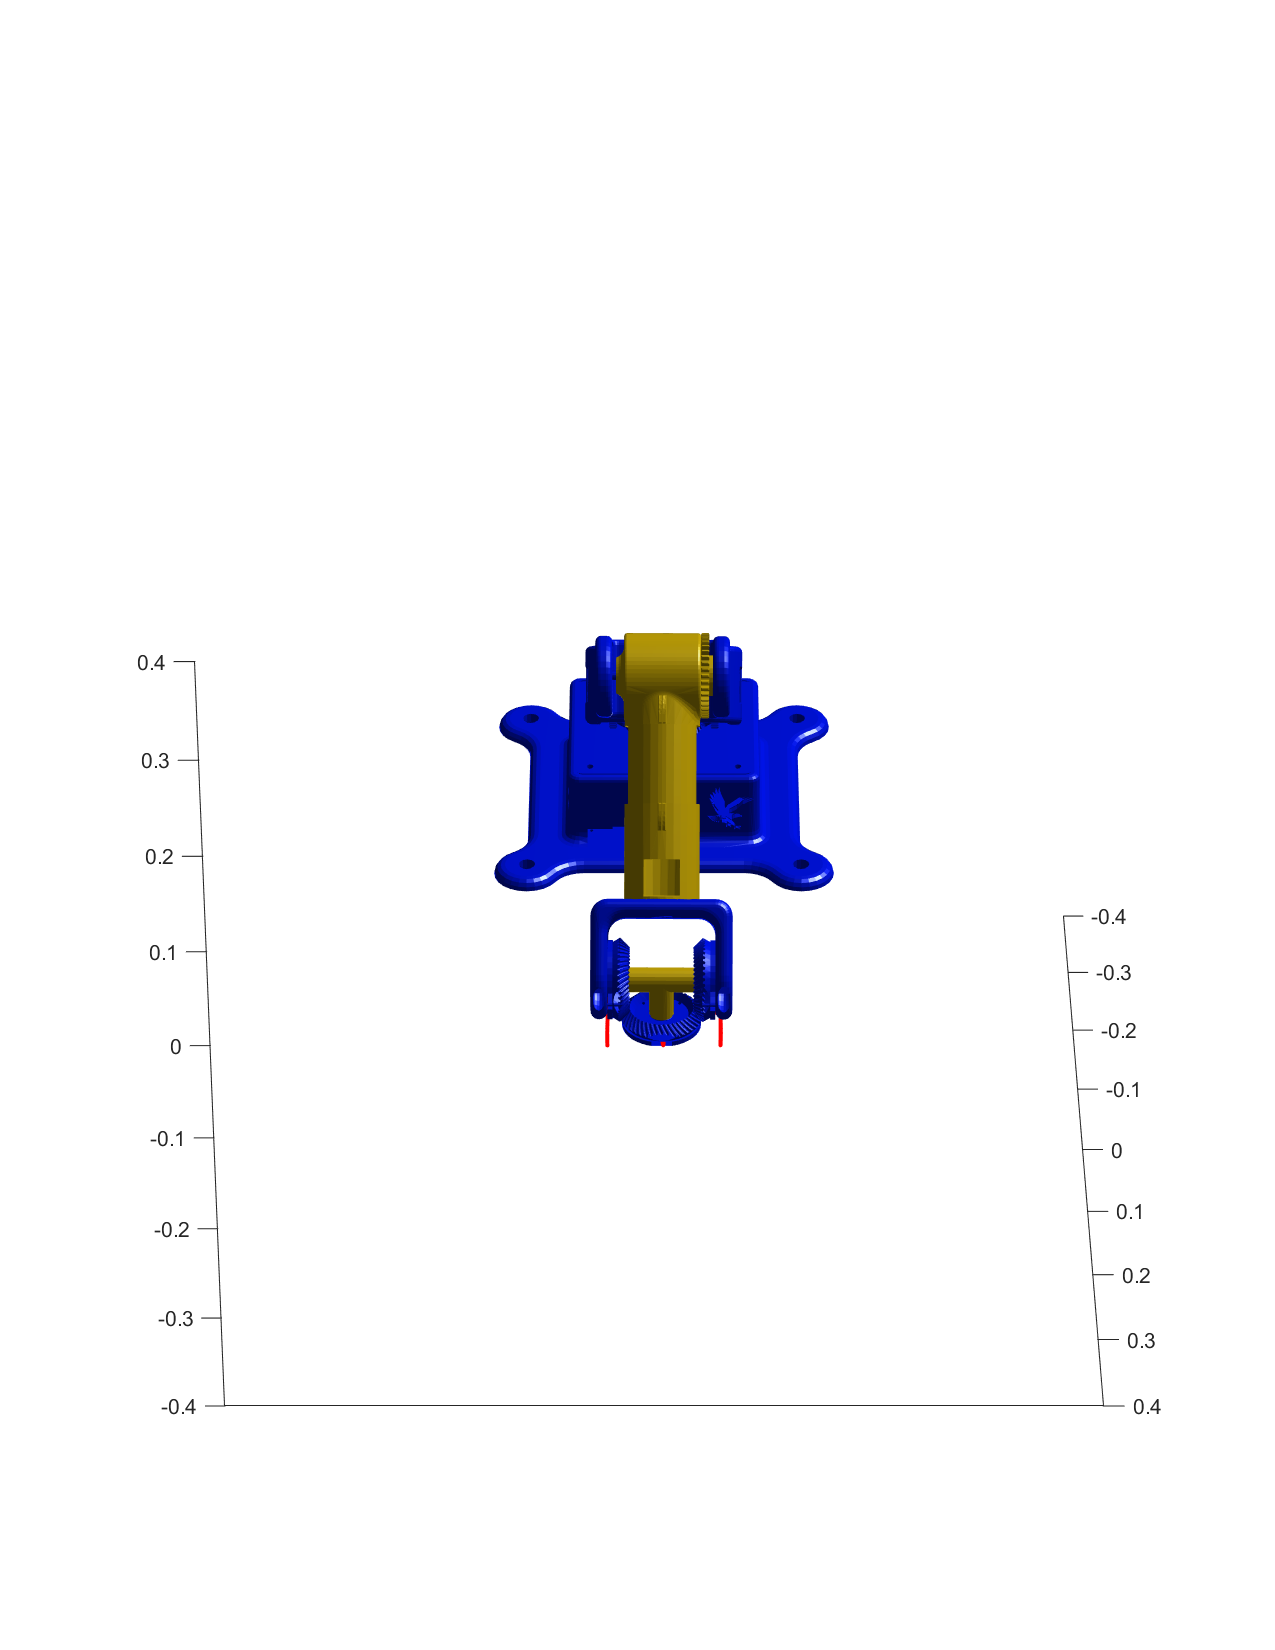
\includegraphics[width=.9\textwidth,frame]{clsnap2}
%     \caption{Frame Snapshot near Simulation \\Middle}
%   \end{subfigure}%
% \begin{subfigure}[c]{0.33\textwidth}
%   \center
%   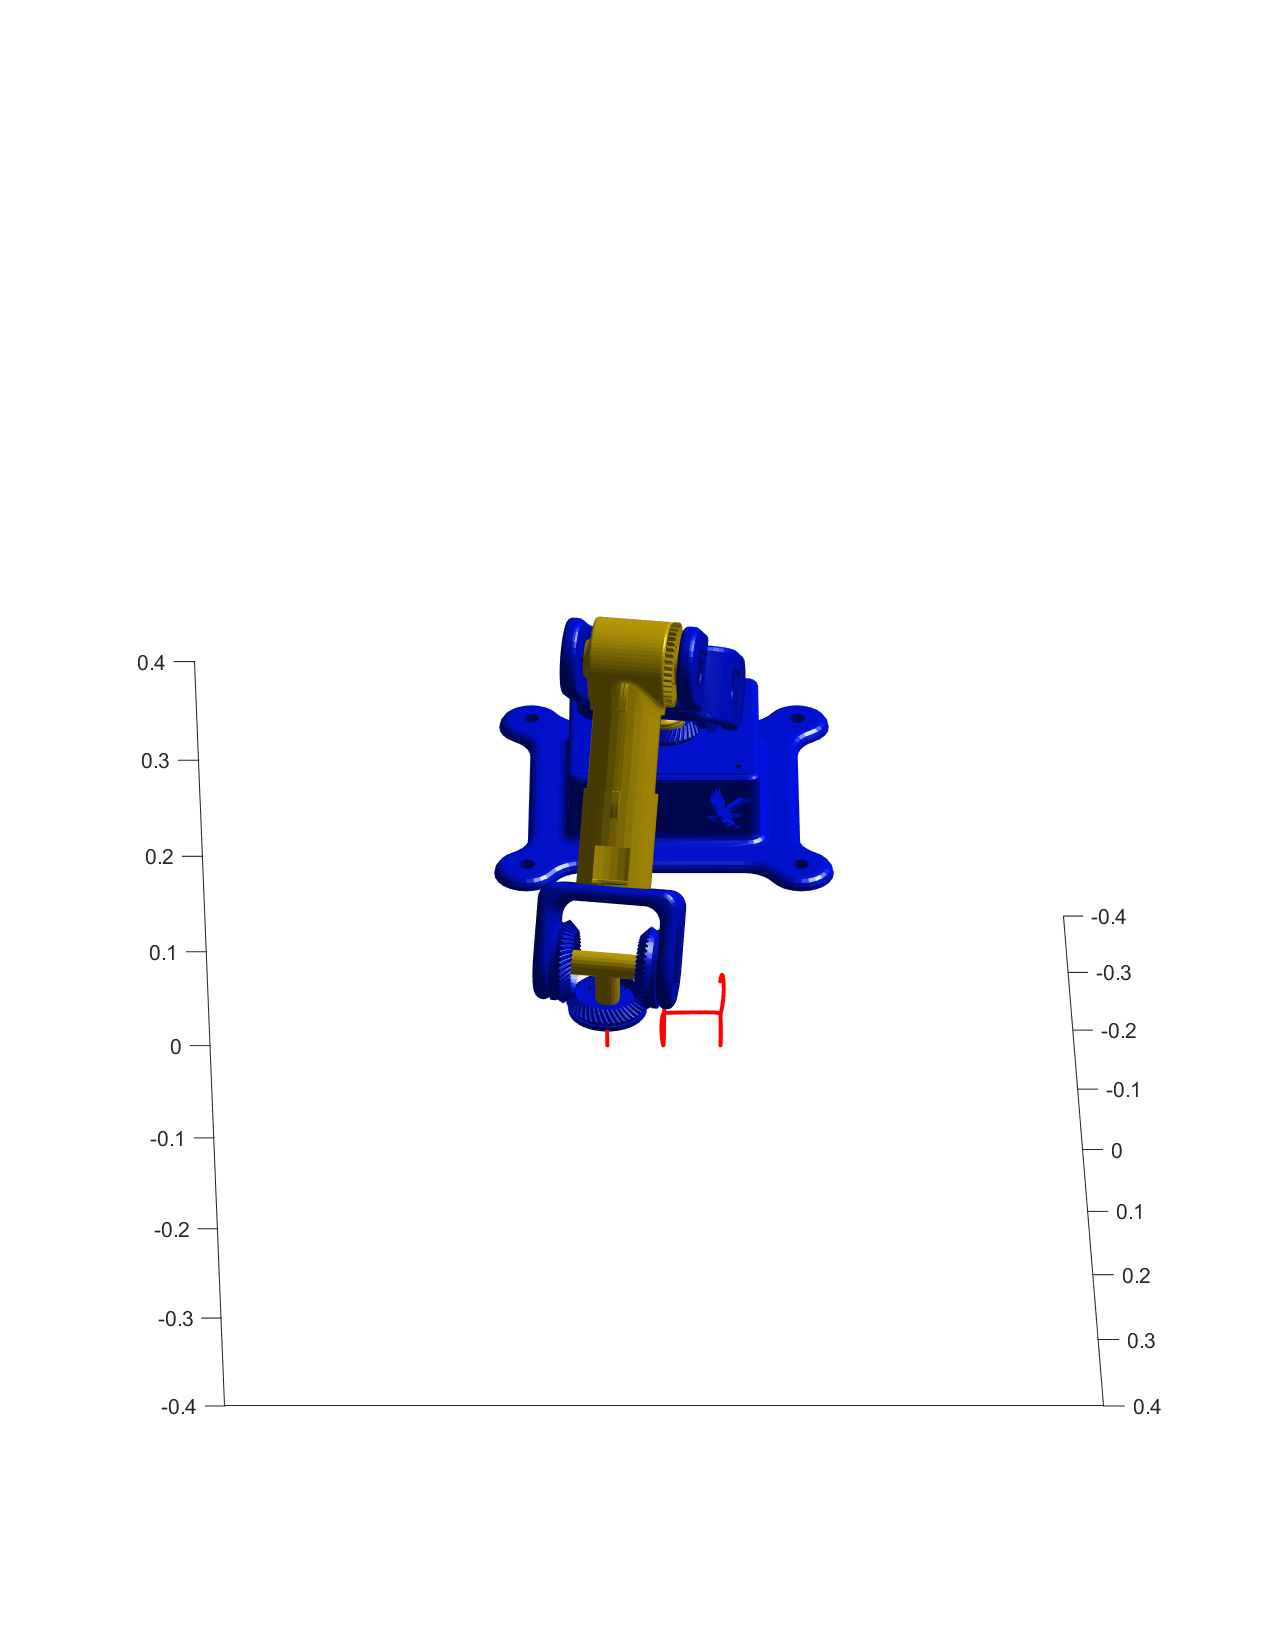
\includegraphics[width=.9\textwidth,frame]{clsnap3}
%   \caption{Frame Snapshot near Simulation \\Termination}
% \end{subfigure}
%   \caption{Closed-Loop Control Simulation Animation Snapshots}
%   \label{fig:clsnaps}
% \end{figure}
%
% \begin{figure}[htp]
%   \center
%   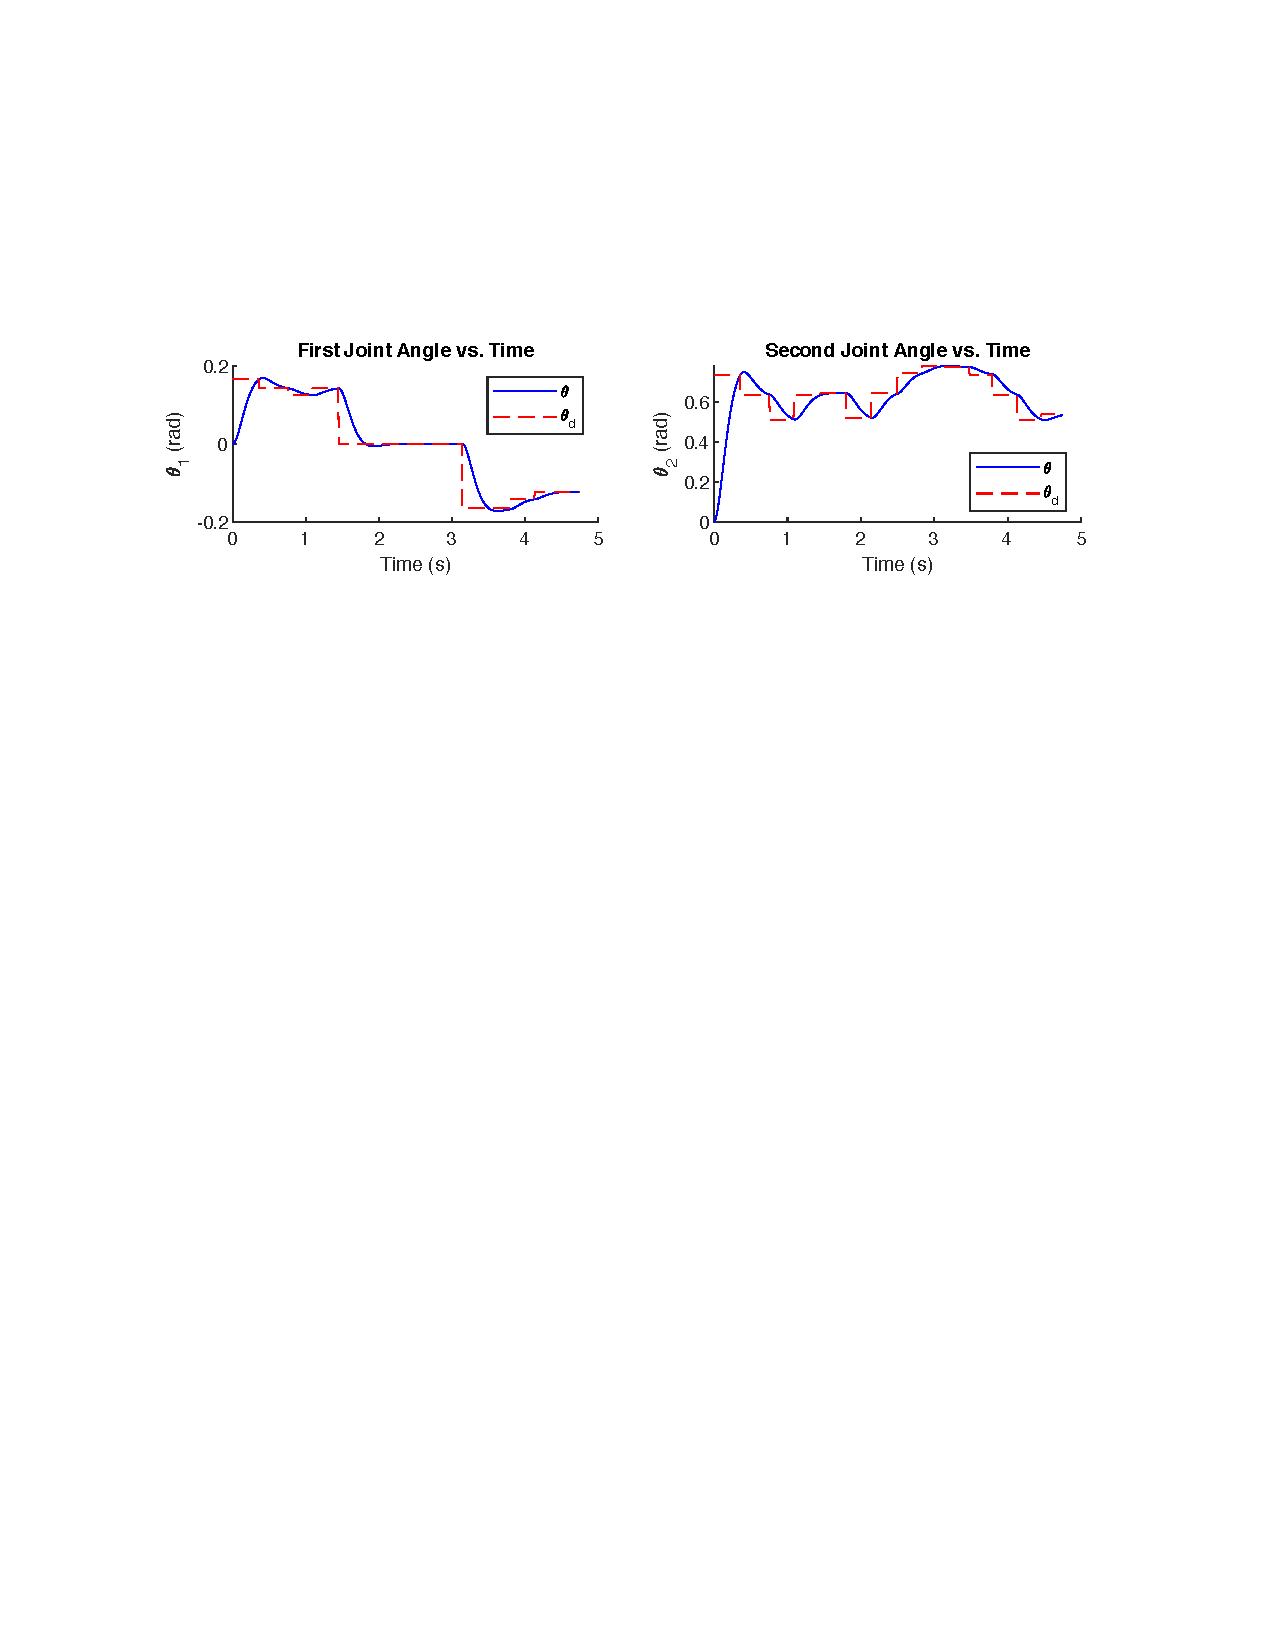
\includegraphics[width=.95\textwidth]{cljplots1}
%   \caption{Joint Angles vs Time in Closed-Loop Simulation}
%   \label{fig:cljplots1}
% \end{figure}
% \begin{figure}[htp]
%   \center
%   \ContinuedFloat
%   \captionsetup{list=off,format=cont}
%   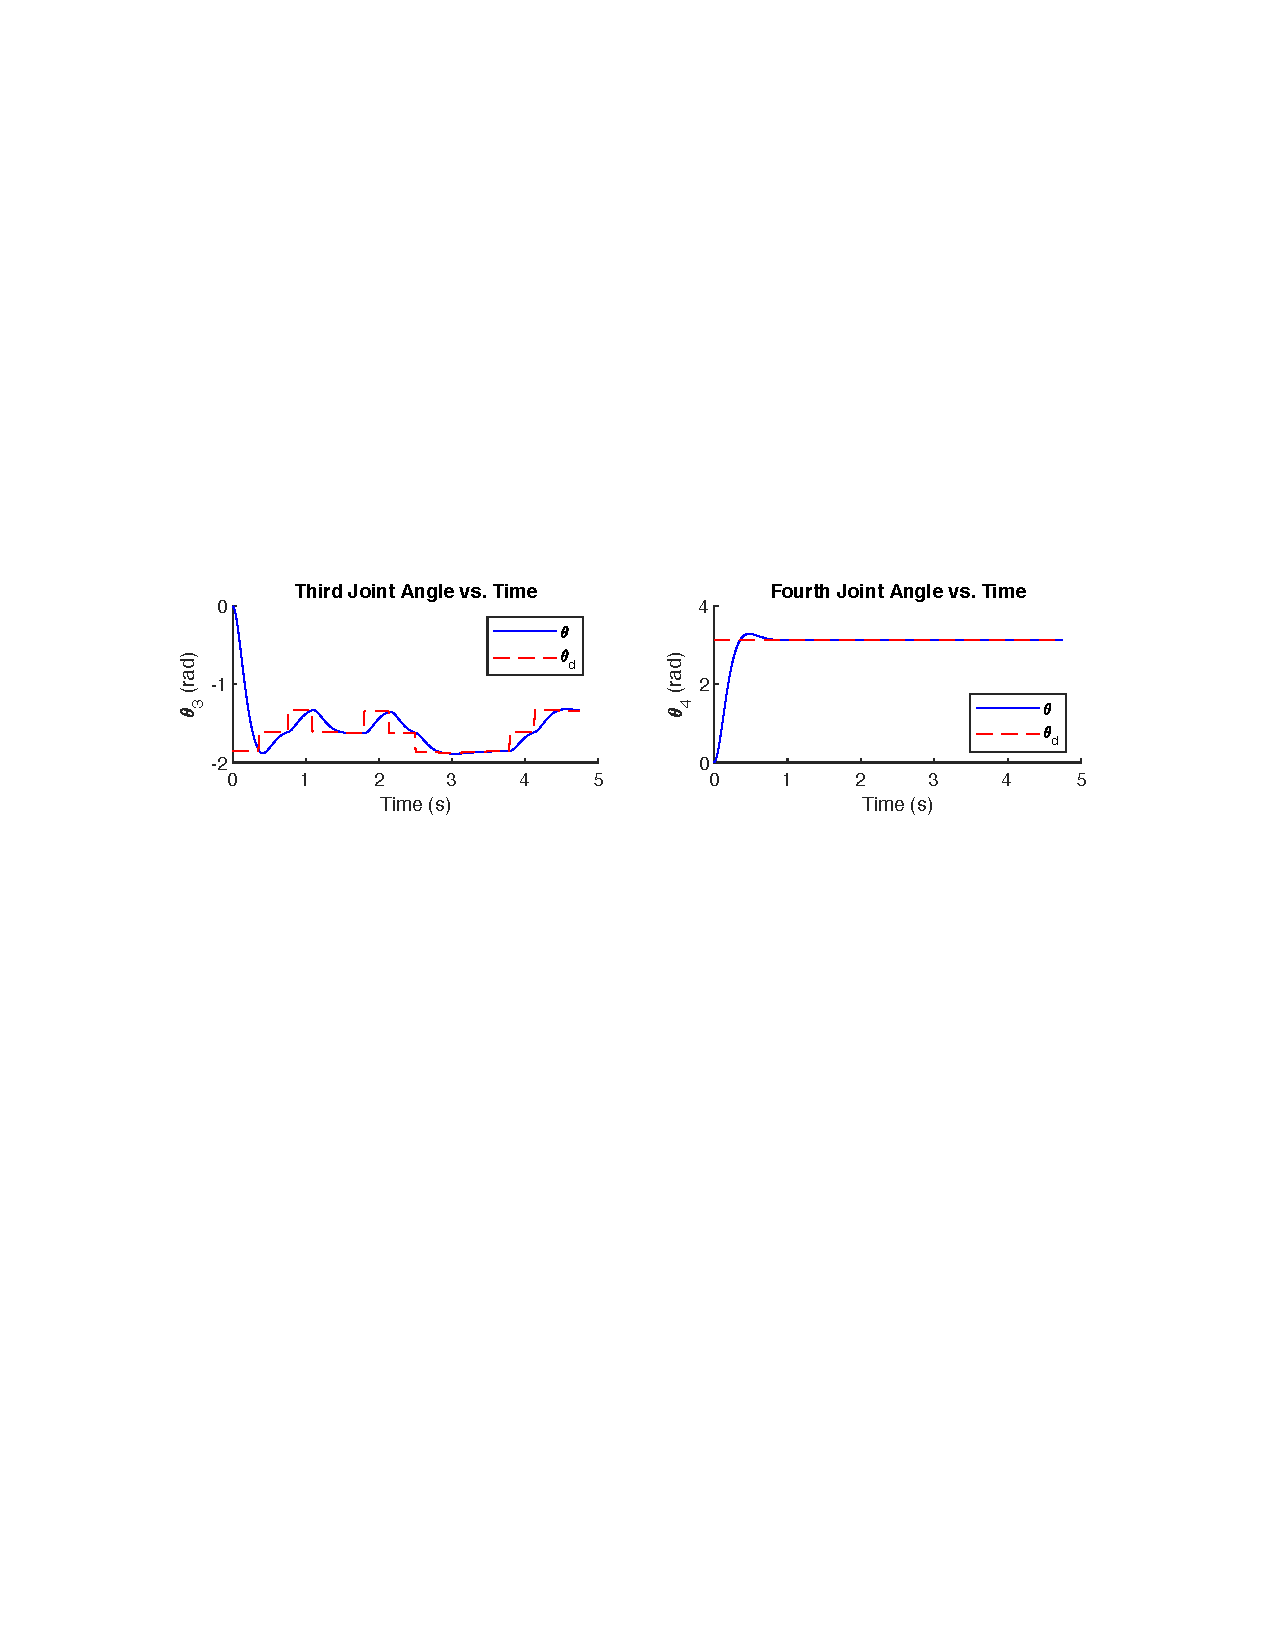
\includegraphics[width=.95\textwidth]{cljplots2}
%   \caption{Joint Angles vs Time in Closed-Loop Simulation}
%   \label{fig:cljplots2}
% \end{figure}
% \begin{figure}[htp]
%   \center
%   \ContinuedFloat
%   \captionsetup{list=off,format=cont}
%   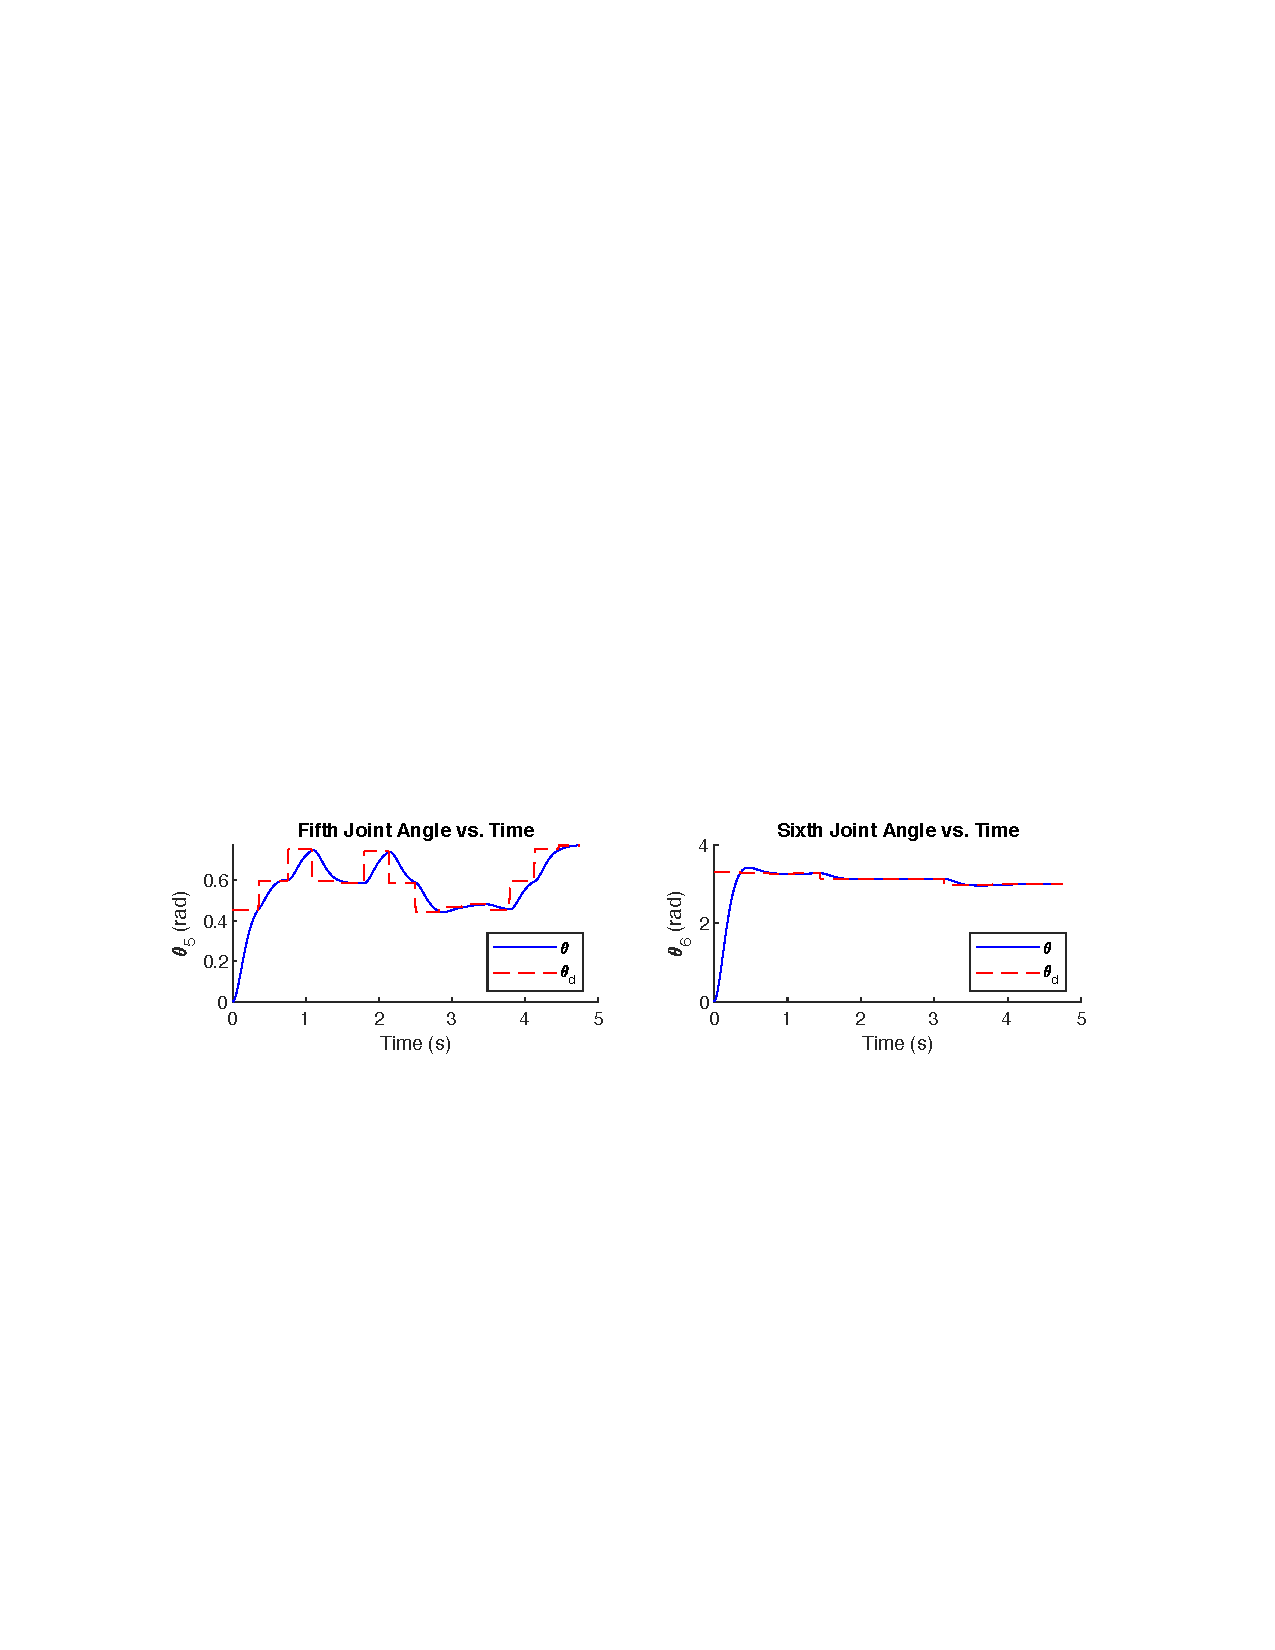
\includegraphics[width=.95\textwidth]{cljplots3}
%   \caption{Joint Angles vs Time in Closed-Loop Simulation}
%   \label{fig:cljplots3}
% \end{figure}
